\chapter{Budowa aplikacji}
\label{ch:budowa_aplikacji}

\section{Moduły i klasy}
\indent \indent W celu uzyskania przejrzystości aplikacji, wydzielone zostały moduły\footnote{W kontekście tej pracy \textit{moduł} oznacza pewną grupę skojarzonych ze sobą klas.}, które opisują pewien fragment funkcjonalności programu. Moduły niższych warstw mogą być wykorzystywane przez moduły warstw wyższych, lub być tylko zestawem dodatkowych narzędzi. Kolejne punkty opisują w czym dany moduł się specjalizuje i\,jakie klasy wchodzą w jego skład. Szczegółowe dane na temat klas oraz ich metod i pól znajdują się w dokumentacji kodu w katalogu {\tt doc}.

\subsection{Komendy}
\indent \indent Klasy komend są tak naprawdę nakładką na istniejące mechanizmy biblioteki ev3dev, operujące bezpośrednio na sprzęcie. Oprócz właściwej komendy, będącej poleceniem dla efektora bądź sensora, dana klasa zawiera referencje do obiektu, na którym ma zostać wykonana oraz jej parametry, o ile takowe posiada. Nazewnictwo klas dokładnie odwzorowuje nazwy komend przekazywanej urządzeniom. W obrębie konkretnych komend, definiowane są także stałe opisujące charakter przekazywanych argumentów oraz ich limity.\\
Komendy zostały podzielone na dwie podgrupy:
\begin{description}
    \item[Komendy motorów:] Klasa bazowa - {\tt CommandMotor}. Zawierają referencje do\,klasy {\tt Motor} oraz opcjonalnie przechowują także przekazywane\\parametry. \\Np przykład: {\tt CommandMotorStop}, {\tt CommandMotorRunForever}.

    \item[Komendy sensorów:] Klasa bazowa - {\tt CommandSensor}. Zawierają referencje do\,klasy {\tt Sensor}. Definiują obsługiwane tryby danego sensora. Komendy te nie służą do pobierania wartości, lecz tylko do zmiany ustawień sensora. Pobieranie wartości używane jest przy pomocy specjalnej klasy {\tt Devices}. \\Przykładowa komenda: {\tt CommandSensorSetMode}.
\end{description}
Klasą bazową dla wszystkich komend jest klasa {\tt Command}.

\subsection{Akcje}
\indent \indent Akcje są kolejnym stopniem abstrakcji definiowania zachowań robota. Klasy akcji przechowują przede wszystkim sekwencje komend, które mają zostać wykonane. Ponadto, z powodu natychmiastowego charakteru wykonywania wszystkich zgromadzonych komend, akcja może mieć zdefiniowany warunek jej zakończenia. Przyjmuje ona postać funkcji anonimowej, w której następuje zwrócenie wartości logicznej na podstawie dowolnie sprecyzowanych instrukcji. Pozwala to wyższej warstwie sterującej sprawdzić, czy kolejna akcja może zostać wykonana. Dodatkowo, akcje mogą deklarować dopuszczalne zdarzenia, które przerywają jej działanie lub zmieniają jej parametry.

Wszystkie dostępne klasy akcji są zdefiniowane w aplikacji i nie istnieje możliwość zwiększenia zbioru o nowe bądź dynamicznego generowania nowych, własnych klas. Ta decyzja implementacyjna jest podyktowana specyfiką konkretnych modeli robotów, różniących się budową oraz podłączonymi akcesoriami, a co za tym idzie, odmiennym sposobem implementacji tych samych czynności.

Klasy opisujące konkretne akcje, np. {\tt ActionDriveDistance}, dziedziczą po klasie {\tt Action}. Wspólnymi elementami każdej z nich są: typ, warunek końcowy, sekwencja komend oraz metody wykonawcze. Różnią się natomiast dodatkowymi parametrami, takimi jak prędkość czy kąt obrotu. Ponadto, istnieje możliwość wygodnego zapętlenia jednej lub wielu akcji dowolną liczbę razy za pomocą specjalnej klasy - {\tt ActionRepeat}. Konstruktor tej klasy przyjmuje liczbę powtórzeń oraz listę akcji, które zostaną wykonane w podanej kolejności.

\begin{figure}[!ht]
    \centering
        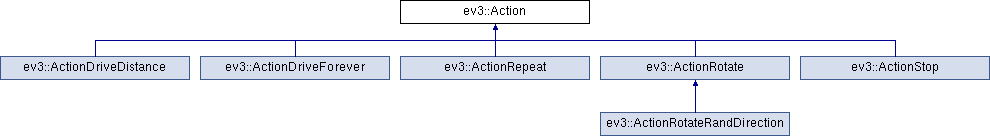
\includegraphics[width=1\textwidth]{diagrams/action_class.png}
    \caption{Diagram dziedziczenia klas akcji.\label{fig:action_class}}
\end{figure}

\subsection{Zachowania}

\indent \indent Definiowanie zachowań jest dużo trudniejsze niż akcji czy komend, gdyż bazują one na schemacie automatu skończonego. Oprócz konkretnych akcji, na jakich dane zachowanie ma się opierać, należy zdefiniować przejścia pomiędzy stanami (akcjami) w toku poprawnego wykonania oraz specjalne warunki zmiany stanu w\,reakcji na zaistniałe zdarzenia (np. napotkana przeszkoda lub utrata połączenia).

Podobnie jak w przypadku akcji i komend, każde zachowanie zdefiniowane jest w osobnej klasie (np. {\tt BehaviourExplore}), które dziedziczy po wspólnej klasie {\tt Behaviour}. Każde z nich zawiera typ, strukturę stanów automatu złożonych z\,akcji i przejść oraz funkcje wykonawcze. Ponadto zachowania pochodne zawierają własne parametry, np. maksymalny dystans do przejechania. Więcej szczegółów w\,rozdziale~\ref{ch:zachowania}. \hyperref[ch:zachowania]{Zachowania}.

\begin{figure}[!ht]
    \centering
        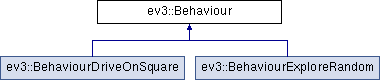
\includegraphics[width=0.5\textwidth]{diagrams/behaviour_class.png}
    \caption{Diagram dziedziczenia klas zachowań.\label{fig:behaviour_class}}
\end{figure}

\subsection{Urządzenia}

\indent \indent Biblioteka ev3dev dostarcza wygodnego interfejsu do zarządzania urządzeniami przez wygenerowanie drzew klas dla sensorów i efektorów. W ramach tej aplikacji, na każdy typ urządzenia została nałożona specjalna klasa pośrednicząca, w\,środku której znajduje się referencja do właściwego obiektu. Są to klasy {\tt Motor} oraz {\tt Sensor}, które po odpowiedniej identyfikacji zostają zmapowane do par port-urządzenie.

Całością nadzoruje klasa {\tt Devices} napisana zgodnie ze wzorcem projektowym \gls{singleton}. Ograniczone są w ten sposób nadmierne kopie obiektów i potencjalnie niejednoznaczne odwołania. Ponadto klasy urządzeń są potrzebne w wielu różnych miejscach aplikacji, a wzorzec ten umożliwia taki dostęp za pomocą statycznego wydobycia instancji.

Moduł urządzeń jest także odpowiedzialny za detekcję zdarzeń. Wyższe warstwy mogą zgłaszać zdarzenia, na które klasa {\tt Devices} ma nasłuchiwać. Jeśli dane zdarzenie wystąpi, wysyłane jest do odpowiedniej kolejki dla wyższych warstw do\,przetworzenia. Zgłaszane mogą być również zdarzenie niezależne, np. niski poziom baterii lub odłączenie urządzenia.

\subsection{Robot}

\indent \indent Jest to najbardziej rozbudowana klasa, ponieważ agreguje w sobie działanie wielu modułów. Zarządza zarówno urządzeniami podłączonymi do klocka centralnego, steruje zachowaniem robota oraz przetwarza przesłane komunikaty i zdarzenia. Podstawowa metoda klasy {\tt run} jest uruchamiana w głównym wątku aplikacji i w pętli przetwarza wszystkie dane. Jest bezpośrednio zsynchronizowana z wątkiem komunikacyjnym za pomocą dwóch kolejek wiadomości - nadawczej i\,odbiorczej. Wyróżnienie dwóch niezależnych ścieżek wykonania umożliwia lepsze zarządzanie zasobami sprzętowymi oraz pozwala robotowi na samodzielne działanie, niezależnie od przesyłanych pakietów.

Robot może być fizycznie zbudowany na wiele różnych sposobów. Dlatego wymagane jest, żeby zdefiniowane były konkretne klasy implementujące szczegóły danego modelu. W związku z powyższym, klasa bazowa {\tt Robot} jest klasą abstrakcyjną, a każdemu wariantowi konstrukcji odpowiada osobna klasa podrzędna. W\,celu ujednolicenia interfejsu, każdy model deklaruje listę obsługiwanych akcji oraz\,wymaganych do tego podłączonych urządzeń. W ten sposób można łatwo sprawdzić, czy dane zachowanie jest obsługiwane i jakich pomiarów robot może dostarczyć. Klasy konkretnych modeli, bazując na istniejących funkcjach wirtualnych, definiują swoje wersje w sposób adekwatny do domniemanego efektu końcowego wymaganych akcji.

Każda instancja robota posiada również maszynę stanów oraz zdefiniowane warunki przejść pomiędzy nimi. Każdy stan przetwarza tylko konkretne komunikaty i\,zdarzenia. Rezultatem ich przetworzenia może być wysłanie specjalnej wiadomości zwrotnej lub zmiana stanu na inny. To ostanie wiąże się jeszcze ze zmianą koloru oraz częstotliwości migania diod LED umieszczonych na przednim panelu klocka centralnego. Możliwe stany przedstawia diagram \ref{fig:robot_states}.

\begin{figure}[!ht]
    \centering
        \includegraphics[width=0.75\textwidth]{diagrams/robot_states.png}
    \caption{Diagram przejść stanów robota. Przerywana linia oznacza migające diody w kolorze stanu, ciągła stałe świecenie.\label{fig:robot_states}}
\end{figure}

\subsection{Komunikacja}

\indent \indent Komunikacja pomiędzy różnymi partiami całego systemu odbywa się na dwóch poziomach:

\subsubsection{Zdarzenia}

Poszczególne moduły robota, takie jak akcje czy klasa urządzeń, mogą generować zdarzenia. Kolejka zdarzeń posiada wiele punktów wejścia, ale tylko jedno wyjście - klasę {\tt Robot}. Wszystkie klasy zdarzeń dziedziczą po klasie {\tt Event}. Zgłaszane do\,kolejki obiekty mogą dotyczyć zarówno zmian wartości sensorów, niespodziewanych zmian w przebiegu zachowania lub wyjątków rzuconych przez aplikację. Więcej szczegółów w rozdziale~\ref{ch:komunikacja}. \hyperref[ch:komunikacja]{Komunikacja}.

\subsubsection{Protokół UDP}

Komunikacja pomiędzy robotami odbywa się przy użyciu sieci bezprzewodowej oraz protokołu UDP. Każdy wysłany pakiet to zakodowany do postaci znakowej obiekt klasy {\tt Message}. Każdy z nich zawiera pięć elementów: identyfikator wiadomości, nadawcy i odbiorcy, typ oraz listę opcjonalnych parametrów. Separatorem parametrów jest dwukropek. Podstawą ustalenia szczegółów wiadomości jest jej identyfikator oraz typ. Pierwszy komponent zapewnia synchronizację pakietów oraz eliminację duplikatów, a drugi steruje zmianami stanów agenta oraz jego zachowań. Więcej szczegółów w rozdziale~\ref{ch:komunikacja}. \hyperref[ch:komunikacja]{Komunikacja}.

\subsection{Nadzorca}

Do poprawnej i kontrolowanej pracy całego systemu potrzebny jest jego nadzorca. Ten wyspecjalizowany moduł zarządza pozostałymi agentami, będąc punktem wspólnym komunikacji wszystkich jednostek. Pozwala mu to na rozdzielanie zachowań dla poszczególnych robotów, synchronizację komunikacji oraz zbieranie danych. Nadzorcą może być zarówno robot LEGO jak i dowolny komputer osobisy, co w tym drugim przypadku umożliwia wykorzystanie większej mocy obliczeniowej.

Za kontrolę systemu odpowiada klasa {\tt Master}. Podobnie jak klasa {\tt Robot}, zawiera ona dwie kolejki do wymiany wiadomości z pracującym równolegle wątkiem komunikacji. Oprócz tego, przechowuje ona informacje o\,wszystkich agentach w\,specjalnej klasie {\tt Agent}, która odpowiada konkretnemu fizycznemu robotowi, ale\,jest pozbawiona wszystkich komponentów sterujących zachowaniami. Jej głównymi atrybutami są identyfikator urządzenia oraz identyfikator wiadomości. Pierwszy z\,nich przydzielany jest agentowi, gdy ten po raz pierwszy nawiążę połączenie z nadzorcą. Drugi z kolei wykorzystywany jest do synchronizacji przesyłanych pakietów w celu dobierania par zapytanie-odpowiedź oraz pomaga usunąć nadmiarowe duplikaty.

Największym problemem przed jakim mogą stanąć roboty (w krytycznej sytuacji - wszystkie jednocześnie), to utrata połączenia z nadzorcą. Szczegóły takiego zdarzenia opisane są w sekcji~\ref{sec:utrata_polaczenia} \hyperref[sec:utrata_polaczenia]{Utrata połączenia z nadzorcą}.

\subsection{Moduły dodatkowe}

Główne klasy aplikacji są wspierane przez dodatkowe, mniej znaczące moduły. Do\,takich należą:

\subsubsection{Kontrola diod LED}

Klasa {\tt LedControl} powstała z konieczności, ponieważ dostarczony interfejs poprawnie obsługiwał tylko jedną z czterech dostępnych diod. Dostarczono zatem metod, które pozwalają sterować jasnością konkretnych diod, wybierać kolor oraz zlecać miganie z odpowiednim interwałem. Klasa ta jest głównie wykorzystywana do wizualnej identyfikacji stanu, w jakim obecnie znajduje się robot.

\subsubsection{Logowanie}

Zarówno w procesie tworzenia aplikacji, jak i w późniejszym jej użytkowaniu, informacje o przebiegu wykonania są niezbędne. Klasa {\tt Logger} pozwala zdefiniować poziom obsługiwanych komunikatów, od bardzo rozwlekłego (verbose) do zawężonego tylko do błędów (error). Ponadto, można wyznaczyć domyślny strumień wyjściowych danych, taki jak standardowe wyjście bądź zapis do pliku. W przypadku zapisywania wiadomości na dysk, dane są gromadzone w paczce i zrzucane na nośnik co pewien interwał, w celu ograniczenia ilości operacji dyskowych.

\subsubsection{Obsługa sygnałów}

Aplikacja musi obsługiwać dostarczane do niej sygnały i poprawnie na nie reagować. Przy starcie programu, tworzony jest obiekt klasy {\tt SignalHandler}, który odwołując się obiektów sterujących, wysyła żądanie zatrzymania po otrzymaniu konkretnych sygnałów.

\subsubsection{Kolejki i bufory}

Zarówno komunikacja wewnętrzna jak i zewnętrzna, korzysta z specjalnych klas do przesyłania oraz przechowywania danych. W przypadku wiadomości, wątek główny i komunikacyjny korzystają z synchronizowanych obiektów klasy szablonowej {\tt Queue}, która implementuje dobrze znaną kolejkę wraz z obslugą współbieżności. Klasa {\tt EventQueue}, stworzona w oparciu o wzorzez \gls{singleton}, implementuje kolejkę obiektów typu {\tt Event}. Ostatnią kolekcją danych jest klasa szablonowa {\tt CircularBuffer}, implementująca bufor cykliczny z nałożonym limitem obiektów w nim przechowywanych. Wykorzystywana głównie w wątku komunikacyjnym do\,eliminacji nadmiarowych pakietów.

Przepływ danych został przedstawiony na rysunkach \ref{fig:event_queue} i \ref{fig:queue}.

\begin{figure}[!ht]
    \centering
        \includegraphics[width=0.75\textwidth]{diagrams/event_queue.png}
    \caption{Kolejka zdarzeń. Wiele klas generujących zdarzenia odbierane przez\,klasę Robot.\label{fig:event_queue}}
\end{figure}

\begin{figure}[!ht]
    \centering
        \includegraphics[width=0.75\textwidth]{diagrams/queue.png}
    \caption{Synchronizacja wiadomości pomiędzy wątkami za pomocą kolejek wiadomości.\label{fig:queue}}
\end{figure}

\subsubsection{Inne}

Do innych, mniej znaczących elementów należy plik {\tt Utils}, zawierający statyczne definicje powszechnie wykorzystywanych metod, stałych i uproszczonych nazw typów danych, a także klasa {\tt ColorUtils} wspomagająca kolorowanie wiadomości logowanych na ekran.
